\documentclass[11pt]{article}

\usepackage{fullpage,fourier,amsmath,amssymb}
\usepackage{listings,color,url,hyperref}
\usepackage{mdframed,xspace}
\usepackage{epigraph}
\usepackage[x11names]{xcolor}
\usepackage{gensymb}
\usepackage{blkarray}
\usepackage{wrapfig}


\usepackage{fancyhdr}
\pagestyle{fancy}
\fancyhf{}

\fancypagestyle{plain}{%
  \fancyhf{}
  \renewcommand{\headrulewidth}{0pt}
  \renewcommand{\footrulewidth}{0pt}
  \lfoot{\textcopyright{} 2021 Darrell Long}
  \rfoot{\thepage}
}

\pagestyle{plain}

\definecolor{codegreen}{rgb}{0,0.5,0}
\definecolor{codegray}{rgb}{0.5,0.5,0.5}
\definecolor{codepurple}{rgb}{0.58,0,0.82}

\lstloadlanguages{C,make,python,fortran}

\lstdefinestyle{c99}{
    morekeywords={bool, uint8_t, uint16_t, uint32_t, uint64_t, int8_t, int16_t, int32_t, int64_t},
    commentstyle=\color{codegreen},
    keywordstyle=\color{magenta},
    numberstyle=\tiny\color{codegray},
    identifierstyle=\color{blue},
    stringstyle=\color{codepurple},
    basicstyle=\ttfamily,
    breakatwhitespace=false,
    breaklines=true,
    captionpos=b,
    keepspaces=true,
    numbers=left,
    numbersep=5pt,
    showspaces=false,
    showstringspaces=false,
    showtabs=false,
    tabsize=4
}

\newenvironment{funcdoc}[1]{\subsubsection*{\underline{\textbf{\texttt{#1}}}}}{}

\newcommand{\monkey}[1]{
  \begin{center}
    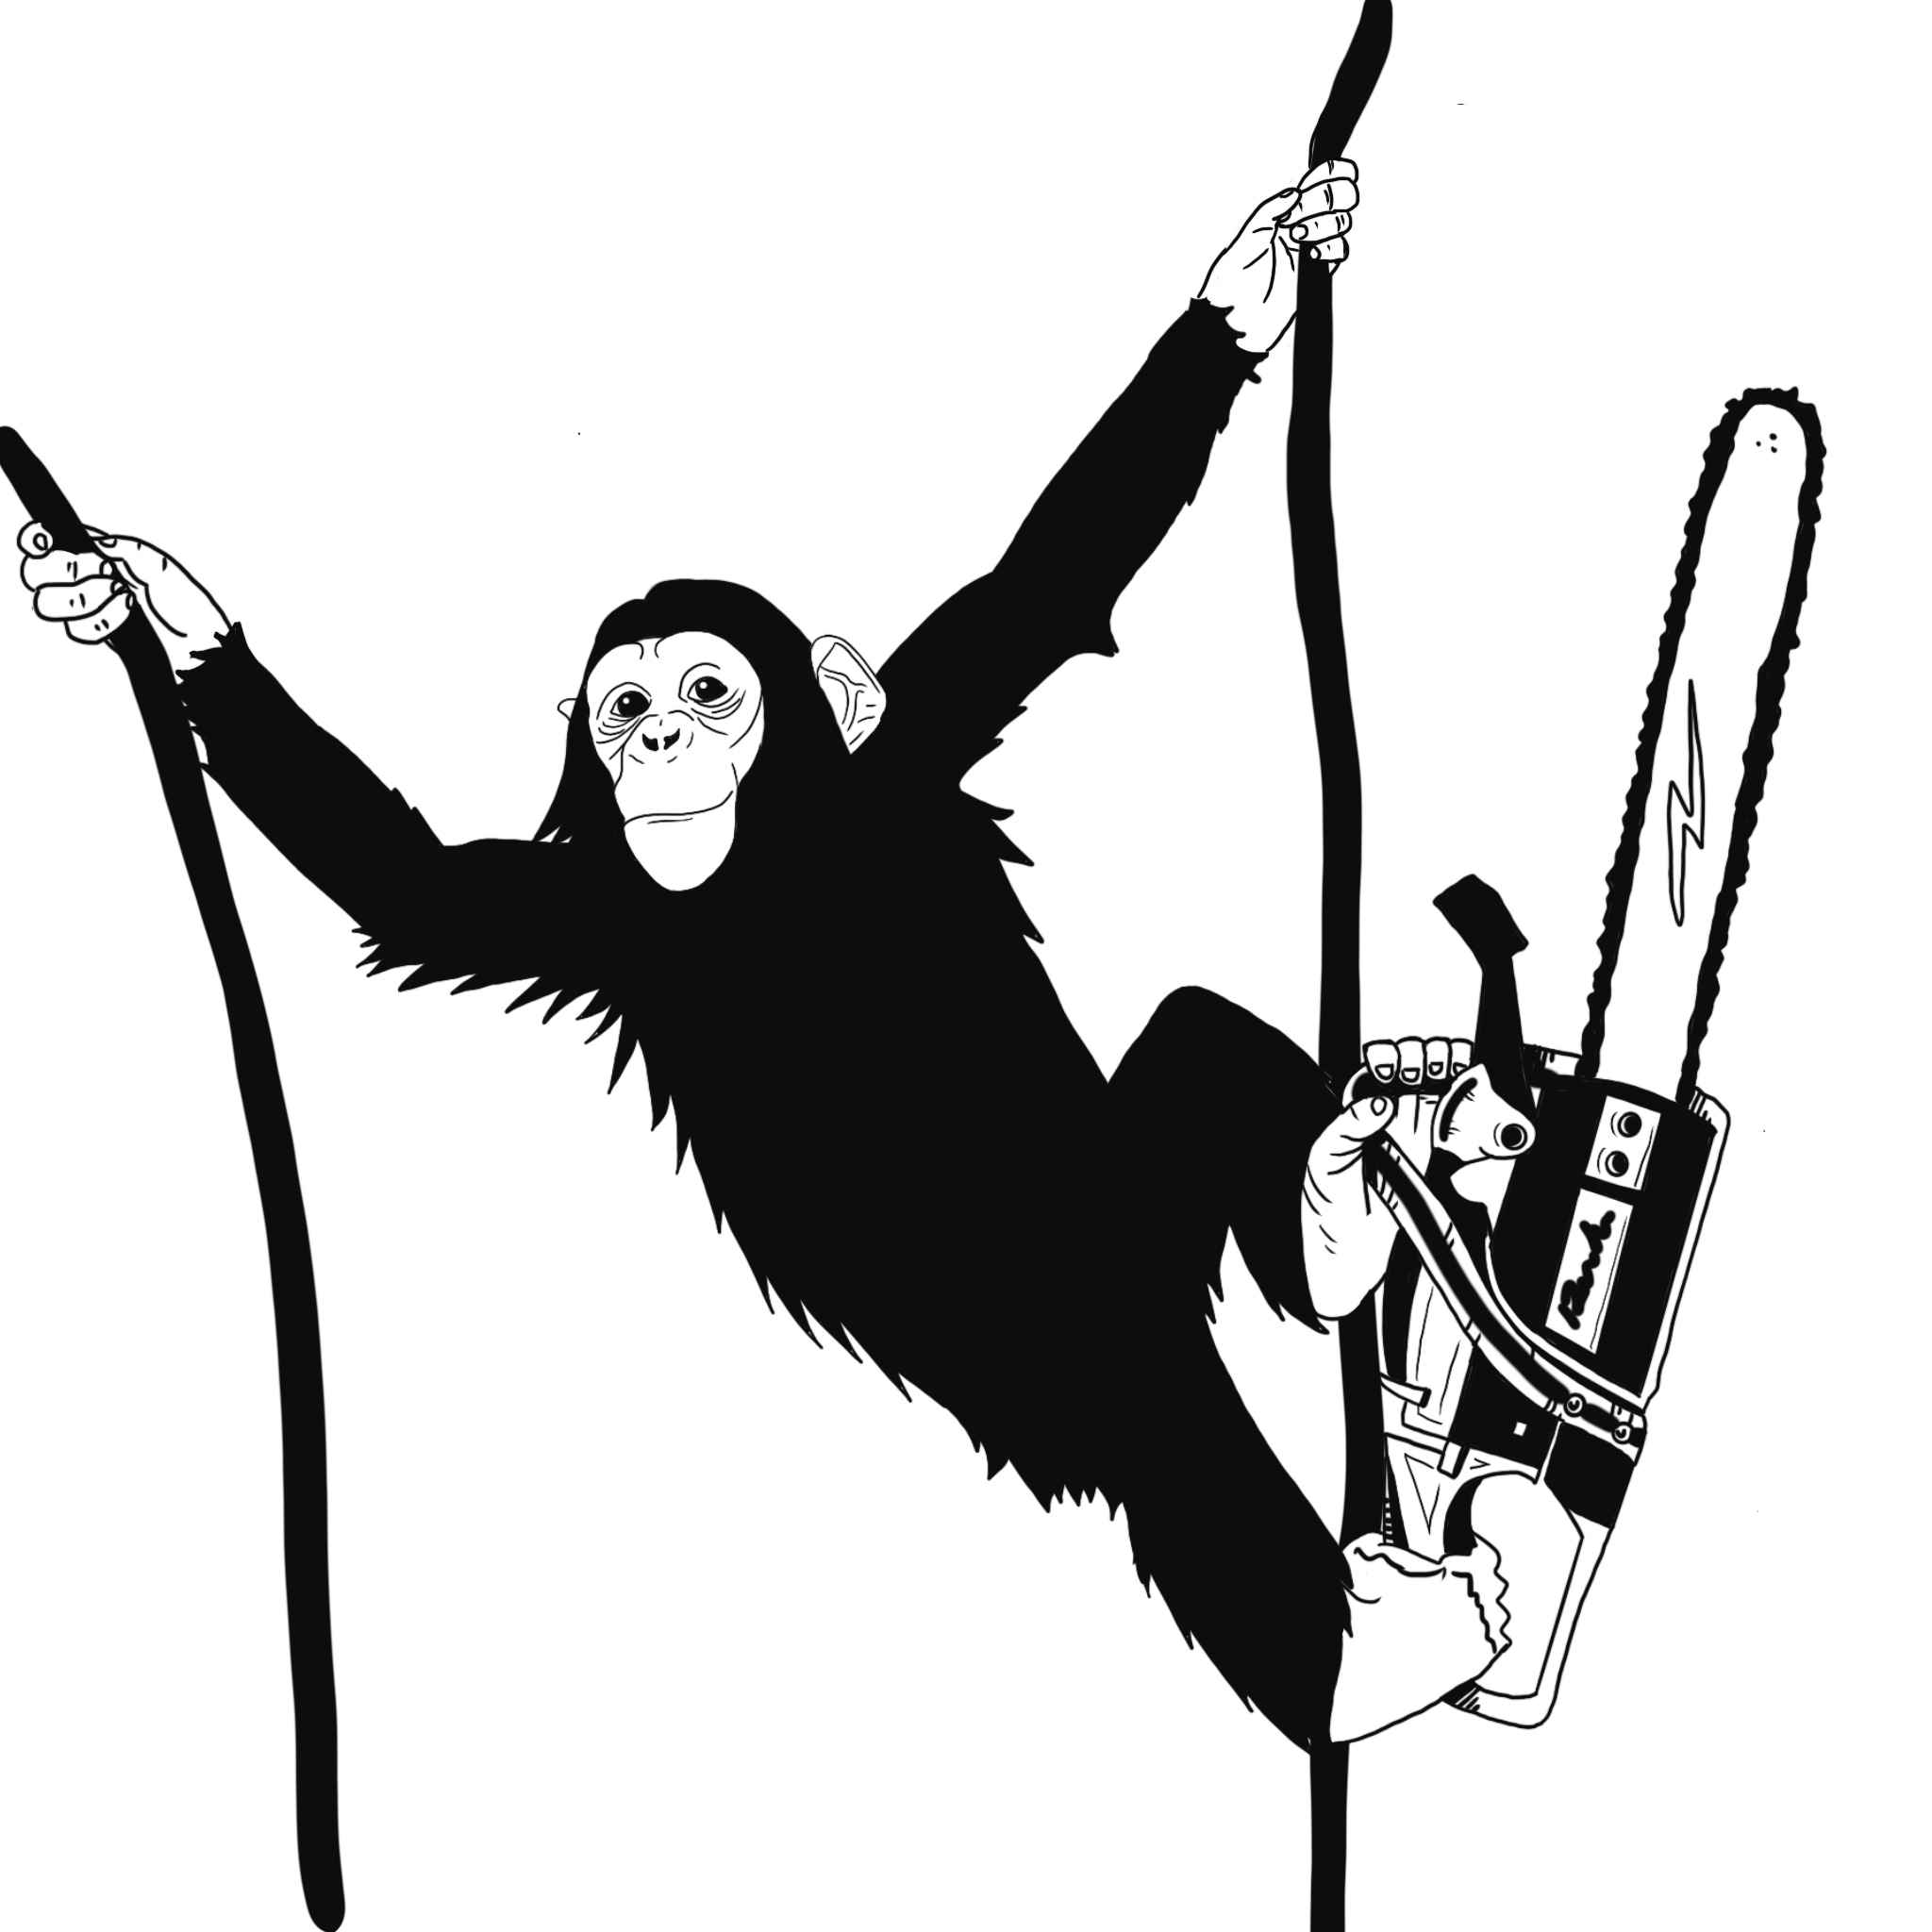
\includegraphics[width=0.35\textwidth]{../monkey.jpg} \\
    \emph{#1}
  \end{center}
}


\title{Assignment 4 \\ The Perambulations of Denver Long \\ \bigskip
\centerline{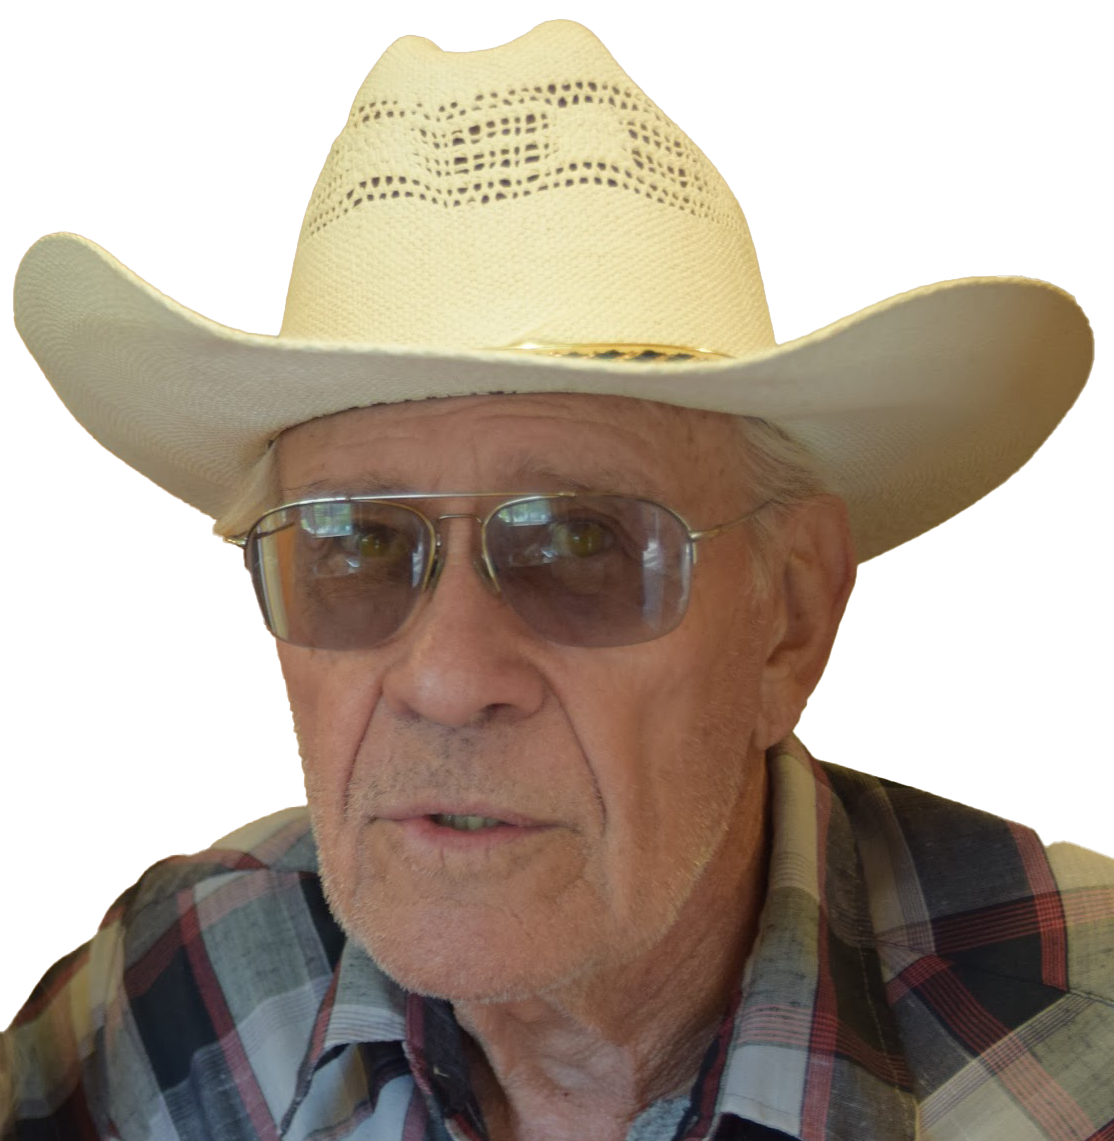
\includegraphics[width=0.3\textwidth]{images/DDL.png}}}
\author{Prof. Darrell Long \\ CSE 13S -- Fall 2021}
\date{Due: October 24$^\text{th}$ at 11:59\,pm}

\begin{document}

\maketitle

\section{Introduction}

\epigraphwidth=0.65\textwidth
\epigraph{\emph{I wonder why it is that when I plan a route too
    carefully, it goes to pieces, whereas if I blunder along in blissful
    ignorance aimed in a fancied direction I get through with no
    trouble.}}{---John Steinbeck, \emph{Travels with Charley: In Search
    of America}}

\noindent
Denver Long decided to augment his income during his retirement
years by selling the prestigious products produced by the Shinola
Corporation.  He enjoys driving his Cadillac, so it's the life of
a traveling salesman for him.  He loads up his little dog Satan---whom
he calls \emph{Baby}---and heads out on his new career.

But his first trip does not go so well. Heading to his son's house
after visiting his new grandson, he accidentally takes a wrong turn
near Chula Vista and winds up in Mexico.  Despite many pleasant
visits to Tijuana in years past, visiting his old friend Se\~nor Vasquez
on his ranchero, shooting their rifles at an old El Dorado that he has traded to Se\~nor
Vasquez decades before,
it's no longer the familiar Mexico of 1974.  Having
no passport, and speaking very little Spanish, he turns around in
frustration.  The Border Patrol won't let him back into the United
States for many hours, until he finally wears them down through his
power of persuasion.

Since the profit of his new enterprise depends
on the cost and duration of travel, and losing a day in Tijuana
cost him a potential sale in Barstow, he asks his eldest son to
have his class create a computer program that will provide an optimal
route to all the cities along his way and then return him to his
home in scenic Clearlake.

\section{Directed Graphs}

\epigraph{\emph{I mean, if 10 years from now, when you are doing
something quick and dirty, you suddenly visualize that I am looking over
your shoulders and say to yourself ``Dijkstra would not have liked
this,'' well, that would be enough immortality for me.}}{%
---Edsger W.\xspace Dijkstra}

\noindent A graph is a data structure $G = \langle V, E \rangle$ where
$V = \{ v_0, \ldots, v_n \}$ is the set of vertices (or nodes) and $E =
\left \{ \langle v_i,v_j \rangle, \ldots \right \}$ is the set of edges
that connect the vertices. For example, you might have a set of cities
$V = \{ \text{El Cajon}, \text{La Mesa}, \text{San Diego}, \ldots,
\text{La Jolla} \}$ as the vertices and write ``El Cajon'' $\rightarrow$
``Lakeside'' to indicate that there is a path (Los Coches Road) from El
Cajon to Lakeside. If there is a path from El Cajon to Lakeside, as well
as a path from Lakeside to El Cajon, then the edge connecting El Cajon
and Lakeside is \emph{undirected}.

% \begin{wrapfigure}{r}{0.145\textwidth}
% \centering
%   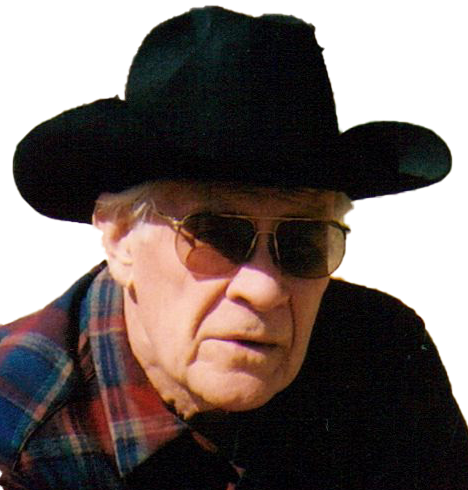
\includegraphics[width=0.14\textwidth]{images/DDL-blk.png}
% \end{wrapfigure}

Such a simple graph representation simply tells you how vertices are
connected and provides the idea of one-way roads. But it really does not
help Denver, since it does not provide any notion of distance. We solve
this problem by associating a weight with each edge and so we might
write ``Santee $\rightarrow$ El Cajon, 2'' to indicate that there is a
path of two miles long from Santee to El Cajon. Given a set of edges and
weights, then we can then find the shortest path from any vertex to any
other vertex (the answer may be that there is no such path). There are
elegant (and quick) algorithms for computing the shortest path, but that
is not exactly what we want to do. We want to find a path through all
of the vertices, visiting each \emph{exactly once}, such that there is a
direct (single step) connection from the last vertex to the first. This
is called a \emph{Hamiltonian path}. This will address Denver's need to
get home, but won't necessarily be the shortest such path. So, we need
to go through every possible Hamiltonian path given the list of cities
Denver is traveling through and pick the shortest path. Note: if you
find yourself on a path that is longer than the current best found
Hamiltonian path, then you can preemptively reject your current path.

\section{Representing Graphs}

\epigraphwidth=0.65\textwidth
\epigraph{\emph{We live on a placid island of ignorance in the midst of
black seas of infinity, and it was not meant that we should voyage
far.}}{---H.\xspace P.\xspace Lovecraft, \emph{The Call of Cthulhu}}

\noindent Perhaps the simplest way to represent a graph is with an
\emph{adjacency matrix}. Consider an $n \times n$ adjacency matrix $M$,
where $n$ is the number of vertices in the graph. If $M_{i,j} = k$,
where $1 \le i \le j \le n$, then we say that there exists a
\emph{directed edge} from vertex $i$ to vertex $j$ with weight $k$.
Traveling through wormholes is considered hazardous, so any valid edge
weight $k$ must be non-zero and positive.

\begin{center}
\begin{blockarray}{ccccccccc}
 & 0 & 1 & 2 & 3 & 4 & 5 & $\dotsi$ & 25\\
\begin{block}{c[>{\medspace}cccccccc<{\medspace}]}
    0 & 0 & 10 & 0 & 0 & 0 & 0 & 0 & 0 \\
    1 & 0 & 0 & 2 & 5 & 0 & 0 & 0 & 0 \\
    2 & 0 & 0 & 0 & 0 & 0 & 3 & 0 & 5 \\
    3 & 0 & 0 & 0 & 0 & 21 & 0 & 0 & 0 \\
    4 & 0 & 0 & 0 & 0 & 0 & 0 & 0 & 0 \\
    5 & 0 & 0 & 0 & 0 & 0 & 0 & 0 & 0 \\
    \smash{\vdots} & 0 & 0 & 0 & 0 & 0 & 0 & 0 & 0 \\
    25 & 0 & 0 & 0 & 0 & 0 & 0 & 0 & 0 \\
\end{block}
\end{blockarray}
\end{center}

\newcommand{\edge}[3]{\langle #1,#2,#3 \rangle}

\noindent Each edge will be represented as a triple $\edge{i}{j}{k}$. The set of
edges in the adjacency matrix above is
\[
E = \left \{
  \edge{0}{1}{10},
  \edge{1}{2}{2},
  \edge{1}{3}{5},
  \edge{2}{5}{3},
  \edge{2}{25}{5},
  \edge{3}{4}{21}
\right \}.
\]

\noindent If the above adjacency matrix were made to be \emph{undirected}, it
would be reflected along the diagonal.

\begin{center}
\begin{blockarray}{ccccccccc}
 & 0 & 1 & 2 & 3 & 4 & 5 & $\dotsi$ & 25\\
\begin{block}{c[>{\medspace}cccccccc<{\medspace}]}
    0 & 0 & 10 & 0 & 0 & 0 & 0 & 0 & 0 \\
    1 & 10 & 0 & 2 & 5 & 0 & 0 & 0 & 0 \\
    2 & 0 & 2 & 0 & 0 & 0 & 3 & 0 & 5 \\
    3 & 0 & 5 & 0 & 0 & 21 & 0 & 0 & 0 \\
    4 & 0 & 0 & 0 & 21 & 0 & 0 & 0 & 0 \\
    5 & 0 & 0 & 3 & 0 & 0 & 0 & 0 & 0 \\
    \smash{\vdots} & 0 & 0 & 0 & 0 & 0 & 0 & 0 & 0 \\
    25 & 0 & 0 & 5 & 0 & 0 & 0 & 0 & 0 \\
\end{block}
\end{blockarray}
\end{center}

\noindent The first of the ADTs you will need to implement for this
assignment is for the graph. An \textbf{ADT} is an \emph{abstract data
type}. With any ADT comes an interface comprised of \emph{constructor},
\emph{destructor}, \emph{accessor}, and \emph{manipulator} functions.

\begin{clisting}{}
struct Graph {
    uint32_t vertices;                   // Number of vertices.
    bool undirected;                     // Undirected graph?
    bool visited[VERTICES];              // Where have we gone?
    uint32_t matrix[VERTICES][VERTICES]; // Adjacency matrix.
};
\end{clisting}

We elect to use an adjacency matrix with set maximum dimensions. This is
both to simplify the abstraction and also due to the computational
complexity of solving the Traveling Salesman Problem (TSP) with
depth-first search (DFS), which is discussed in \S 5. The
\texttt{VERTICES} macro will be defined and supplied to you in
\texttt{vertices.h}. In this header file, there is another macro
\texttt{START\_VERTEX} which defines the origin vertex of the shortest
Hamiltonian path we will be searching for. \textcolor{red}{You may not
modify this file. The \texttt{struct} definition of a graph \emph{must}
go in \texttt{graph.c}.}
\begin{clisting}{\texttt{vertices.h}}
#pragma once

#define START_VERTEX 0   // Starting (origin) vertex.
#define VERTICES     26  // Maximum vertices in graph.
\end{clisting}

The interface for the graph ADT is defined as
follows:

\begin{funcdoc}{Graph *graph\_create(uint32\_t vertices, bool undirected)}
  The constructor for a graph. A constructor function is responsible for
  initializing and allocating any memory required for the type it is
  constructing. It is through this constructor in which a graph can be
  specified to be undirected. Make sure each cell of the adjacency
  matrix, \texttt{matrix}, is set to zero. Also make sure that each
  index of the \texttt{visited} array is initialized as \texttt{false}
  to reflect that no vertex has been visited yet. The \texttt{vertices}
  field reflects the number of vertices in the graph. A working
  constructor for a graph is provided below. Note that it uses
  \texttt{calloc()} for \emph{dynamic memory allocation}. This function
  is included in \texttt{<stdlib.h>}.

  \begin{clisting}{}
Graph *graph_create(uint32_t vertices, bool undirected) {
    Graph *G = (Graph *)calloc(1, sizeof(Graph));
    G->vertices = vertices;
    G->undirected = undirected;
    return G;
}
  \end{clisting}

\end{funcdoc}

\begin{funcdoc}{void graph\_delete(Graph **G)}
  The destructor for a graph. A working destructor for a \texttt{Graph}
  is provided below. Any memory that is allocated using one of
  \texttt{malloc()}, \texttt{realloc()}, or \texttt{calloc()}
  \emph{must} be freed using the \texttt{free()} function. The job of
  the destructor is to free all the memory allocated by the constructor.
  \textcolor{red}{Your programs are expected to be free of memory
  leaks.} A pointer to a pointer is used as the parameter because we
  want to avoid \emph{use-after-free} errors. A use-after-free error
  occurs when a program uses a pointer that points to freed memory. To
  avoid this, we pass the \emph{address of a pointer} to the destructor
  function. By \emph{dereferencing} this double pointer, we can make
  sure that the pointer that pointed to allocated memory is updated to
  be \texttt{NULL}.

  \begin{clisting}{}
void graph_delete(Graph **G) {
    free(*G);
    *G = NULL;
    return;
}
  \end{clisting}
\end{funcdoc}

\begin{funcdoc}{uint32\_t graph\_vertices(Graph *G)}
  Since we will be using \texttt{typedef} to create \emph{opaque} data
  types, we need functions to access fields of a data type. These
  functions are called \emph{accessor} functions. An opaque data type
  means that users do not need to know its implementation outside of the
  implementation itself. This also means that it is incorrect to write
  \texttt{G->vertices} outside of \texttt{graph.c} since it violates
  opacity. This accessor function returns the number of vertices in the
  graph.
\end{funcdoc}

\begin{funcdoc}{bool graph\_add\_edge(Graph *G, uint32\_t i, uint32\_t j, uint32\_t k)}
  The need for \emph{manipulator} functions follows the rationale behind
  the need for accessor functions: there needs to be some way to alter
  fields of a data type.

  This function adds an edge of weight \texttt{k}
  from vertex \texttt{i} to vertex \texttt{j}. If the graph is
  undirected, add an edge, also with weight \texttt{k} from \texttt{j}
  to \texttt{i}. Return \texttt{true} if both vertices are within bounds
  and the edge(s) are successfully added and \texttt{false} otherwise.
\end{funcdoc}

\begin{funcdoc}{bool graph\_has\_edge(Graph *G, uint32\_t i, uint32\_t j)}
  Return \texttt{true} if vertices \texttt{i} and \texttt{j} are within
  bounds and there exists an edge from \texttt{i} to \texttt{j}. Remember:
  an edge exists if it has a non-zero, positive weight. Return
  \texttt{false} otherwise.
\end{funcdoc}

\begin{funcdoc}{uint32\_t graph\_edge\_weight(Graph *G, uint32\_t i, uint32\_t j)}
  Return the weight of the edge from vertex \texttt{i} to vertex
  \texttt{j}. If either \texttt{i} or \texttt{j} aren't within bounds, or
  if an edge doesn't exist, return 0.
\end{funcdoc}

\begin{funcdoc}{bool graph\_visited(Graph *G, uint32\_t v)}
  Return \texttt{true} if vertex \texttt{v} has been visited and
  \texttt{false} otherwise.
\end{funcdoc}

\begin{funcdoc}{void graph\_mark\_visited(Graph *G, uint32\_t v)}
  If vertex \texttt{v} is within bounds, mark \texttt{v} as visited.
\end{funcdoc}

\begin{funcdoc}{void graph\_mark\_unvisited(Graph *G, uint32\_t v)}
  If vertex \texttt{v} is within bounds, mark \texttt{v} as unvisited.
\end{funcdoc}

\begin{funcdoc}{void graph\_print(Graph *G)}
  A debug function you will want to write to make sure your graph ADT
  works as expected.
\end{funcdoc}

\section{Depth-first Search}

\epigraphwidth=0.65\textwidth \epigraph{\emph{Again it might have been
the American tendency in travel. One goes, not so much to see but to
tell afterward.}}{---John Steinbeck, \emph{Travels with Charley: In
Search of Amerca}}

\noindent
We need a methodical procedure for searching through the graph. Once we
have examined a vertex, we do not want to do so again---we don't want
Denver going through cities where he has already been (he has been known
to wear out his welcome: charming women and fighting men).

Depth-first search (DFS) first marks the vertex $v$ as having been visited,
then it iterates through all of the edges $\langle v, w \rangle$,
recursively calling itself starting at $w$ if $w$ has not already been
visited.

\begin{clisting}{}
procedure DFS(G,v):
    label v as visited
    for all edges from v to w in G.adjacentEdges(v) do
       if vertex w is not labeled as visited then
          recursively call DFS(G,w)
    label v as unvisited
\end{clisting}

Finding a Hamiltonian path then reduces to:
\begin{enumerate}
\item
Using DFS to find paths that pass through all vertices, and
\item
There is an edge from the last vertex to the first. The solutions to the
Traveling Salesman Problem are then the shortest found Hamiltonian
paths.
\end{enumerate}

\section{Computational Complexity}

\epigraphwidth=0.65\textwidth \epigraph{\emph{Many a trip continues long
    after movement in time and space have ceased. I remember a man in
    Salinas who in his middle years traveled to Honolulu and back, and
    that journey continued for the rest of his life. We could watch him
    in his rocking chair on his front porch, his eyes squinted,
    half-closed, endlessly traveling to Honolulu.}}{---John Steinbeck,
    \emph{Travels with Charley: In Search of Amerca}}

\noindent
How long will this take?
The answer is, it will take a very long time if there are a large number
of vertices. The running time of the simplest algorithm is
$\operatorname{O}(n!)$ and there is no known algorithm that runs in less
than $\operatorname{O}(2^n)$ time.  In fact, the TSP has been shown to
be NP-hard, which means that it is as difficult as any problem in the
class NP (you will learn more about this in CSE\,104: Computability and
Computational Complexity).  Basically, it means that it can be solved in
polynomial time if you have a magical computer that at each if-statement
is takes both branches every time (creating a copy of the computer for
each such branch).

\section{Stacks}
\epigraphwidth=0.25\textwidth
\epigraph{\emph{The future is unwritten.}}{---Joe Strummer}

You will need to use a \emph{stack} in your decoder to reconstruct a
Huffman tree. The interface of the stack should be familiar from
assignment 4. The difference is that the stack this time around will
store \emph{nodes}. The interface for the stack is defined in
\texttt{stack.h}.

\begin{clisting}{}
struct Stack {
    uint32_t top;
    uint32_t capacity;
    Node **items;
};
\end{clisting}

\begin{funcdoc}{\texttt{Stack *stack\_create(uint32\_t capacity)}}
  The constructor for a stack. The maximum number of nodes the stack can
  hold is specified by \texttt{capacity}.
\end{funcdoc}

\begin{funcdoc}{\texttt{void stack\_delete(Stack **s)}}
  The destructor for a stack. Remember to set the pointer to \texttt{NULL}
  after you free the memory allocated by the stack.
\end{funcdoc}

\begin{funcdoc}{\texttt{bool stack\_empty(Stack *s)}}
  Returns \texttt{true} if the stack is empty and \texttt{false}
  otherwise.
\end{funcdoc}

\begin{funcdoc}{\texttt{bool stack\_full(Stack *s)}}
  Returns \texttt{true} if the stack is full and \texttt{false} otherwise.
\end{funcdoc}

\begin{funcdoc}{\texttt{uint32\_t stack\_size(Stack *s)}}
  Returns the number of nodes in the stack.
\end{funcdoc}

\begin{funcdoc}{\texttt{bool stack\_push(Stack *s, Node *n)}}
  Pushes a node onto the stack. Returns \texttt{false} if the stack is
  full prior to pushing the node and \texttt{true} otherwise to indicate
  the successful pushing of a node.
\end{funcdoc}

\begin{funcdoc}{\texttt{bool stack\_pop(Stack *s, Node **n)}}
  Pops a node off the stack, passing it back through the double pointer
  \texttt{n}. Returns \texttt{false} if the stack is empty prior to
  popping a node and \texttt{true} otherwise to indicate the
  succesuccessful popping of a node.
\end{funcdoc}

\begin{funcdoc}{\texttt{void stack\_print(Stack *s)}}
  A debug function to print the contents of a stack.
\end{funcdoc}

\section{Paths}

\epigraphwidth=0.65\textwidth \epigraph{\emph{We find after years of
struggle that we do not take a trip; a trip takes us.} }{---John
Steinbeck, \emph{Travels with Charley: In Search of Amerca}}

\noindent
Given that vertices are added to and removed from the traveled path in a
stack-like manner, we decide to abstract a path as follows:

\begin{clisting}{}
struct Path {
    Stack *vertices; // The vertices comprising the path.
    uint32_t length; // The total length of the path.
};
\end{clisting}

The following functions define the interface for the path ADT.

\begin{funcdoc}{Path *path\_create(void)}
  The constructor for a path. Set \texttt{vertices} as a freshly created
  stack that can hold up to \texttt{VERTICES} number of vertices.
  Initialize \texttt{length} to be 0. The \texttt{length} field will
  track the length of the path. In other words, it holds the sum of the
  edge weights between consecutive vertices in the \texttt{vertices}
  stack.
\end{funcdoc}

\begin{funcdoc}{void path\_delete(Path **p)}
  The destructor for a path. Remember to set the pointer \texttt{p} to
  \texttt{NULL}.
\end{funcdoc}

\begin{funcdoc}{bool path\_push\_vertex(Path *p, uint32\_t v, Graph
*G)}
Pushes vertex \texttt{v} onto path \texttt{p}. The \texttt{length} of the
path is \emph{increased} by the edge weight connecting the vertex at the top of
the stack and \texttt{v}. Return \texttt{true} if the vertex was
successfully pushed and \texttt{false} otherwise.
\end{funcdoc}

\begin{funcdoc}{bool path\_pop\_vertex(Path *p, uint32\_t *v, Graph
*G)}
  Pops the \texttt{vertices} stack, passing the popped vertex back through
  the pointer \texttt{v}. The \texttt{length} of the path is
  \emph{decreased} by the edge weight connecting the vertex at the top of
  the stack and the popped vertex. Return \texttt{true} if the vertex was
  successfully popped and \texttt{false} otherwise.
\end{funcdoc}

\begin{funcdoc}{uint32\_t path\_vertices(Path *p)}
  Returns the number of vertices in the path.
\end{funcdoc}

\begin{funcdoc}{uint32\_t path\_length(Path *p)}
  Returns the length of the path.
\end{funcdoc}

\begin{funcdoc}{void path\_copy(Path *dst, Path *src)}
  Assuming that the destination path \texttt{dst} is properly initialized,
  makes \texttt{dst} a copy of the source path \texttt{src}. This will
  require making a copy of the \texttt{vertices} stack as well as the
  \texttt{length} of the source path.
\end{funcdoc}

\begin{funcdoc}{void path\_print(Path *p, FILE *outfile, char
*cities[])}
  Prints out a path to \texttt{outfile} using \texttt{fprintf()}. Requires
  a call to \texttt{stack\_print()}, as defined in \S 7.10, in order to
  print out the contents of the \texttt{vertices} stack.
\end{funcdoc}

% \section{Stacks, Revisited}

% \epigraphwidth=0.55\textwidth \epigraph{\emph{I believe that what we become depends on
% what our fathers teach us at odd moments, when they aren't trying to teach us.
% We are formed by little scraps of wisdom.}}{---Umberto Eco, \emph{Foucault's Pendulum}}

% \noindent
% You will use the stack that you implemented for assignment 3 with slight
% modifications. If there were any problems with your stack for that
% assignment, make sure to fix them for this assignment. Here is the
% modified stack interface for this assignment.

% \begin{clisting}{}
% struct Stack {
%     uint32_t top;
%     uint32_t capacity;
%     uint32_t *items;
% };
% \end{clisting}

% \subsection{\texttt{Stack *stack\_create(uint32\_t capacity)}}

% The constructor function for a \texttt{Stack}. The \texttt{top} of a
% stack should be initialized to 0. The capacity of a stack is set to the
% specified capacity. The specified capacity also indicates the number of
% items to allocate memory for, the items in which are held in the
% dynamically allocated array \texttt{items}.

% \subsection{\texttt{void stack\_delete(Stack **s)}}

% The destructor function for a stack. Remember to set the pointer
% \texttt{s} to \texttt{NULL}.

% \subsection{\texttt{bool stack\_empty(Stack *s)}}

% Return \texttt{true} if the stack is empty and \texttt{false} otherwise.

% \subsection{\texttt{bool stack\_full(Stack *s)}}

% Return \texttt{true} if the stack is full and \texttt{false} otherwise.

% \subsection{\texttt{uint32\_t stack\_size(Stack *s)}}

% Return the number of items in the stack.

% \subsection{\texttt{bool stack\_push(Stack *s, uint32\_t x)}}

% If the stack is full prior to pushing the item \texttt{x}, return
% \texttt{false} to indicate failure.  Otherwise, push the item and return
% \texttt{true} to indicate success.

% \subsection{\texttt{bool stack\_peek(Stack *s, uint32\_t *x)}}

% Peeking into a stack is synonymous with querying a stack about the
% element at the top of the stack.  If the stack is empty prior to peeking
% into it, return \texttt{false} to indicate failure.

% \subsection{\texttt{bool stack\_pop(Stack *s, uint32\_t *x)}}

% If the stack is empty prior to popping it, return \texttt{false} to
% indicate failure. Otherwise, pop the item, set the value in the memory
% \texttt{x} is pointing to as the popped item, and return \texttt{true}
% to indicate success.

% \subsection{\texttt{void stack\_copy(Stack *dst, Stack *src)}}

% Assuming that the destination stack \texttt{dst} is properly initialized,
% make \texttt{dst} a copy of the source stack \texttt{src}. This means
% making the \emph{contents} of \texttt{dst->items} the same as
% \texttt{src->items}. The top of \texttt{dst} should also match the top
% of \texttt{src}.

% \subsection{\texttt{void stack\_print(Stack *s, FILE *outfile, char
% *cities[])}}

% Prints out the contents of the stack to \texttt{outfile} using
% \texttt{fprintf()}. Working through each vertex in the stack starting
% from the \emph{bottom}, print out the name of the city each vertex
% corresponds to. This function will be given to aid you.

% \begin{clisting}{}
% void stack_print(Stack *s, FILE *outfile, char *cities[]) {
%     for (uint32_t i = 0; i < s->top; i += 1) {
%         fprintf(outfile, "%s", cities[s->items[i]]);
%         if (i + 1 != s->top) {
%             fprintf(outfile, " -> ");
%         }
%     }
%     fprintf(outfile, "\n");
% }
% \end{clisting}

\section{Command-line Options}

\epigraphwidth=0.65\textwidth
\epigraph{\emph{Attitude is a choice. Happiness is a choice. Optimism is
a choice. Kindness is a choice. Giving is a choice. Respect is a choice.
Whatever choice you make makes you. Choose wisely.}}{---Roy T.\ Bennett,
\emph{The Light in the Heart}}

\noindent
Your program must support any combination of the following command-line
options.

\begin{itemize}
  \item \textbf{\texttt{-h}}\,: Prints out a help message describing the purpose
    of the graph and the command-line options it accepts, exiting the
    program afterwards. Refer to the reference program in the resources
    repo for an idea of what to print.
  \item \textbf{\texttt{-v}}\,: Enables verbose printing. If enabled,
    the program prints out \emph{all} Hamiltonian paths found as well as
    the total number of recursive calls to \texttt{dfs()}.
  \item \textbf{\texttt{-u}}\,: Specifies the graph to be undirected.
  \item \textbf{\texttt{-i infile}}\,: Specify the input file path
    containing the cities and edges of a graph. If not specified, the
    default input should be set as \texttt{stdin}.
  \item \textbf{\texttt{-o outfile}}\,: Specify the output file path to
    print to. If not specified, the default output should be set as
    \texttt{stdout}.
\end{itemize}

\section{I/O}
\epigraphwidth=0.5\textwidth
\epigraph{\emph{
When I was a child I truly loved:
unthinking love as calm and deep
as the North Sea. But I have lived,
and now I do not sleep.}}{---John Gardner, \emph{Grendel}}

\noindent Now that we have covered all the essential ADTs necessary for
the encoder, we will discuss I/O. Instead of the buffered I/O functions
from \texttt{<stdio.h>} that you have become acquainted with in previous
assignments, we will use low-level system calls (\emph{syscalls}) such
as \texttt{read()}, \texttt{write()}, \texttt{open()} and
\texttt{close()}. The former two functions can be included with
\texttt{<unistd.h>} and the latter two can be included with
\texttt{<fcntl.h>}. Functions defined by the following I/O module will
be used by both the encoder and decoder. The interface for the I/O
module will be supplied in \texttt{io.h}. You will notice two
\texttt{extern} variables defined in \texttt{io.h}: \texttt{bytes\_read}
and \texttt{bytes\_written}. These are here for the purposes of
collecting statistics. \textcolor{red}{These two variables \emph{must}
be defined in \texttt{io.c}.}

\begin{funcdoc}{\texttt{int read\_bytes(int infile, uint8\_t *buf, int
nbytes)}}
  This will be a useful wrapper function to perform reads. As you may
  know, the \texttt{read()} syscall \emph{does not} always guarantee
  that it will read all the bytes specified (as is the case with
  \emph{pipes}). For example, a call could be issued to read a a block
  of bytes, but it might only read part of a block. So, we write a
  wrapper function to \emph{loop calls} to \texttt{read()} until we have
  either read all the bytes that were specified (\texttt{nbytes}) into
  the byte buffer \texttt{buf}, or there are no more bytes to read. The
  number of bytes that were read from the input file descriptor,
  \texttt{infile}, is returned. \textcolor{red}{You should use this
  function whenever you need to perform a read.}
\end{funcdoc}

\begin{funcdoc}{\texttt{int write\_bytes(int outfile, uint8\_t *buf, int
nbytes)}}
  This functions is very much the same as \texttt{read\_bytes()}, except
  that it is for looping calls to \texttt{write()}. As you may imagine,
  \texttt{write()} is not guaranteed to write out all the specified
  bytes (\texttt{nbytes}), and so we must loop until we have either
  written out all the bytes specified from the byte buffer \texttt{buf},
  or no bytes were written. The number of bytes written out to the
  output file descriptor, \texttt{outfile}, is returned.
  \textcolor{red}{You should use this function whenever you need to
  perform a write.}
\end{funcdoc}

\begin{funcdoc}{\texttt{bool read\_bit(int infile, uint8\_t *bit)}}
  You should all know by now that it is \emph{not} possible to read a
  single bit from a file. What you \emph{can} do, however, is read in a
  block of bytes into a buffer and dole out bits one at a time. Whenever
  all the bits in the buffer have been doled out, you can simply fill
  the buffer back up again with bytes from \texttt{infile}. This is
  exactly what you will do in this function. You will maintain a
  \texttt{static} buffer of bytes and an index into the buffer that
  tracks which bit to return through the pointer \texttt{bit}. The
  buffer will store \texttt{BLOCK} number of bytes, where \texttt{BLOCK}
  is yet another macro defined in \texttt{defines.h}. This function
  returns \texttt{false} if there are no more bits that can be read and
  \texttt{true} if there are still bits to read. It may help to treat
  the buffer as a \emph{bit vector}.
\end{funcdoc}

\begin{funcdoc}{\texttt{void write\_code(int outfile, Code *c)}}
  The same bit-buffering logic used in \texttt{read\_bit()} will be used
  in here as well. This function will also make use of a \texttt{static}
  buffer (we recommend this buffer to be static to the file, not just
  this function) and an index. Each bit in the code \texttt{c} will be
  buffered into the buffer. The bits will be buffered starting from the
  $0^\text{th}$ bit in \texttt{c}. When the buffer of \texttt{BLOCK}
  bytes is filled with bits, write the contents of the buffer to
  \texttt{outfile}.
\end{funcdoc}

\begin{funcdoc}{\texttt{void flush\_codes(int outfile)}}
  It is not always guaranteed that the buffered codes will align nicely
  with a block, which means that it is possible to have bits leftover in
  the buffer used by \texttt{write\_code()} after the input file has
  been completely encoded. The sole purpose of this function is to write
  out any leftover, buffered bits. Make sure that any extra bits in the
  last byte are zeroed before flushing the codes.
\end{funcdoc}

\section{Specifics}\label{section:specifics}

You will be writing a \C program, and the first thing is to include
the appropriate header files.

\begin{clisting}{Header Files}
#include <stdbool.h> // Gives us the bool data type
#include <stdio.h>   // ... standard I/O
#include <stdlib.h>  // ... strtoul() and other useful things
#include <string.h>  // ... string utilities
#include <unistd.h>  // ... getopt() and other useful things
\end{clisting}

You will need to process the command line arguments.
The \texttt{-p} option determines whether you will print just
\emph{perfect numbers} or all numbers (which is the default).

\begin{clisting}{Command line arguments}
#define DEFAULT_MAXIMUM 1000
#define OPTIONS "pn:"

int main(int argc, char **argv) {
    int n = DEFAULT_MAXIMUM;
    bool imperfect = true;
    int opt;

    while ((opt = getopt(argc, argv, OPTIONS)) != -1) {
        switch (opt) {
        case 'p':
            imperfect = !imperfect;
            break;
        case 'n':
            n = strtoul(optarg, NULL, 10);
            break;
        }
    }
    // Your other code goes here ...
}
\end{clisting}

For each positive integer from the ordered set $n\in\left\{ 2, \ldots, n\right\}$ you will classify it
as \emph{prime}, \emph{perfect}, \emph{deficient} or \emph{abundant}.

You will print the number, followed by a list of all of its
\emph{proper divisors}, followed by its classification.
Classifying a number requires you to determine \emph{all} of its proper divisors.
\begin{itemize}
\item How do you know if a number $n$ is \emph{prime}? It has only
$1$ as a \emph{proper divisor}.

\item How do you know if a number $n$ is \emph{perfect}? The \emph{sum}
of the proper divisors $s(n) = n$.

\item How do you know if a number $n$ is \emph{deficient}? The
\emph{sum} of the proper divisors $s(n) < n$.

\item How do you know if a number $n$ is \emph{abundant}? The
\emph{sum} of the proper divisors $s(n) > n$.

\end{itemize}
You should see a pattern here that you can (and should) exploit.

You will want to keep an array of the proper divisors, alternatively,
you can keep a string of their decimal representation, but that seems inelegant, especially if you are trying for \emph{extra credit}. You will need to
do this because the \texttt{-p} option will prevent printing of all
\emph{imperfect} numbers. You will not know which class a number
falls into until you have examined all divisors.

\begin{shlisting}{Example}
eco :: ./classify -n 20
2 : [1] is prime
3 : [1] is prime
4 : [1, 2] is deficient
5 : [1] is prime
6 : [1, 2, 3] is perfect
7 : [1] is prime
8 : [1, 2, 4] is deficient
9 : [1, 3] is deficient
10 : [1, 2, 5] is deficient
11 : [1] is prime
12 : [1, 2, 3, 4, 6] is abundant
13 : [1] is prime
14 : [1, 2, 7] is deficient
15 : [1, 3, 5] is deficient
16 : [1, 2, 4, 8] is deficient
17 : [1] is prime
18 : [1, 2, 3, 6, 9] is abundant
19 : [1] is prime
20 : [1, 2, 4, 5, 10] is abundant
\end{shlisting}

\begin{shlisting}{Example}
eco :: ./classify -n 10000 -p
6 : [1, 2, 3] is perfect
28 : [1, 2, 4, 7, 14] is perfect
496 : [1, 2, 4, 8, 16, 31, 62, 124, 248] is perfect
8128 : [1, 2, 4, 8, 16, 32, 64, 127, 254, 508, 1016, 2032, 4064] is perfect
\end{shlisting}

\subsection{Executables}

An executable on \Unix{} is just another name for a program. The terms
\emph{program}, \emph{executable}, \emph{executable binary}, and sometimes just
\emph{binary}, all refer to a program that can be run, or \emph{executed}. The
distinction between an plain old executable and an executable binary is in its
representation. An executable binary is platform specific and is simply a file
full of machine code: pure binary. An executable could be a shell script, which
contains readable text. The only thing these two share is that they must have
the executable bit set in order to be run. Refer to the discussion of \Unix{}
file permissions in assignment 0 if you have forgotten what the executable bit
refers to.

\section{Deliverables}

\epigraphwidth=0.4\textwidth
\epigraph{\emph{It is such a sweet temptation \\ It gives such grief relief \\
It is such a false sensation \\ How come that's so hard to believe?}}{---Ray
Wylie Hubbard, \emph{Loco Gringo's Lament}}

You will need to turn in the following source code and header files:

\begin{enumerate}
  \item Your program \emph{must} have the following source and header
    files:
  \begin{itemize}
    \item \texttt{universe.c} implements the \texttt{Universe} ADT.
    \item \texttt{universe.h} specifies the interface to the \texttt{Universe}
      ADT. This file is provided and \emph{may not} be modified.
    \item \texttt{life.c} contains \texttt{main()} and \emph{may}
      contain any other functions necessary to complete your implementation of
      the Game of Life.
  \end{itemize}
\end{enumerate}

You can have other source and header files, but \emph{do not try to be overly
clever}. You will also need to turn in the following:

\begin{enumerate}
  \item \texttt{Makefile}:
    \begin{itemize}
      \item \texttt{CC = clang} must be specified.
      \item \texttt{CFLAGS = -Wall -Wextra -Werror -Wpedantic} must be specified.
      \item \texttt{make} must build the \texttt{life} executable, as should
        \texttt{make all} and \texttt{make life}.
      \item \texttt{make clean} must remove all files that are compiler
        generated.
      \item \texttt{make format} should format all your source code,
        including the header files.
    \end{itemize}
  \item \texttt{README.md}: This must use proper Markdown syntax. It
    must describe how to use your program and \texttt{Makefile}. It
    should also list and explain any command-line options that your
    program accepts. Any false positives reported by \texttt{scan-build}
    should be documented and explained here as well. Note down any known
    bugs or errors in this file as well for the graders.
  \item \texttt{DESIGN.pdf}: This document \emph{must} be a proper
    PDF\@. This design document must describe your design and design
    process for your program with enough detail such that a sufficiently
    knowledgeable programmer would be able to replicate your
    implementation. \textcolor{red}{This does not mean copying your
    entire program in verbatim}. You should instead describe how your
    program works with supporting pseudocode.
  \item \texttt{WRITEUP.pdf}: This document \emph{must} be a proper
    PDF\@. This writeup document must include everything you learned from
    this assignment. Make sure to mention everything in detail while being as precise as possible. How well you explain all the lessons you have learned in this assignment will be really important here. 
\end{enumerate}

\section{Submission}

Refer back assignment 0 for the instructions on how to properly submit
your assignment through \texttt{git}. Remember: \emph{add},
\emph{commit}, and \emph{push}!

\textcolor{red}{Your assignment is turned in \emph{only} after you have
pushed and submitted the commit ID you want graded on Canvas. ``I
forgot to push'' and ``I forgot to submit my commit ID'' are not valid
excuses. It is \emph{highly} recommended to commit and push your changes
\emph{often}.}

\section{Supplemental Readings}

\epigraph{\emph{The more that you read, the more things you will know. The
more that you learn, the more places you'll go.}}{---Dr.\ Seuss}

\begin{itemize}
  \item \textit{The C Programming Language} by Kernighan \& Ritchie
  \begin{itemize}
    \item Chapter 7
    \item Appendix B
  \end{itemize}
  \item \textit{Introduction to Algorithms} by T.\ Cormen, C.\
    Leiserson, R.\ Rivest, \& C.\ Stein
    \begin{itemize}
      \item Chapter 31 \S 31.2, \S 31.3, \S 31.6, \S 31.7, \S 31.8
    \end{itemize}
\end{itemize}


\monkey{Ph'nglui mglw'nafh Cthulhu R'lyeh wgah'nagl fhtagn.}

\end{document}
